\documentclass[a4paper,12pt]{report}

\usepackage{alltt, fancyvrb, url}
\usepackage{graphicx}
\usepackage[utf8]{inputenc}
\usepackage{float}
\usepackage{hyperref}

% Questo commentalo se vuoi scrivere in inglese.
\usepackage[italian]{babel}

\usepackage[italian]{cleveref}

\title{PROGETTO OOP\\``TICKET TO RIDE''}

\author{Bergami Lorenzo\\
Massa Marco\\
Sbaraccani Pietro\\
Spina Orazio}
\date{\today}


\begin{document}

\maketitle

\tableofcontents

\chapter{Analisi}


\section{Requisiti}
Il progetto si propone di realizzare il gioco da tavolo Ticket to Ride, in cui i giocatori devono costruire una rete ferroviaria, collegando le città presenti sul tabellone secondo degli obiettivi forniti dalle carte pescate. L'obiettivo è completare rotte specifiche assegnate tramite Carte Obiettivo segrete, cercando di conquistare più tratte possibile e collegare città specifiche per ottenere punti bonus. Il vincitore è colui che accumula più punti alla fine del gioco. 

\subsubsection{Requisiti funzionali}
Il numero di giocatori sarà variabile (da 2 a 6), giocheranno tutti dalla stessa istanza dell'applicazione alternandosi. 
La partita è suddivisa in varie fasi:
\begin{itemize}
\item Preparazione partita: i giocatori ricevono una Carta Treno per ogni colore e una Carta Obiettivo, che indica una tratta da completare piazzando treni. Ogni giocatore riceve anche 45 Carrozze, entità che permettono di utilizzare la carta Treno sulla mappa.
\item Fase di gioco: ad ogni turno il giocatore pesca dal mazzo di Carte Treno e può scegliere se riempire una Tratta, pescare una Carta Treno o una Carta Obiettivo. Dopodichè deve passare il turno al Giocatore successivo.
\item Terminazione del gioco: la partita termina allo scadere del primo turno in cui almeno un giocatore ha 2 o meno Carrozze. 
\item Resoconto partita: al termine del gioco viene visualizzata una Scoreboard con i punteggi dei singoli giocatori.
\end{itemize}

\subsubsection{Requisiti non funzionali}
\begin{itemize}
	\item L'esperienza di gioco dovrà essere fluida, con una successione rapida di turni.
 \item L'applicazione dovrà essere reattiva ai comandi dei giocatori
 \item L'interfaccia dev'essere comprensibile, intuitiva e user-friendly
 \item I giocatori devono capire intuitivamente che risorse hanno a disposizione e la situazione sulla mappa di gioco
\end{itemize}

\section{Analisi e modello del dominio}

Questo progetto ha l'obiettivo di simulare un match di "Ticket to Ride" tra un numero di entità Giocatore compreso tra 2 e 6. Il gioco prevede l'interazione da diverse entità Giocatore, ognuna delle quali ha a disposizione Carte Treno, Carte Obiettivo (messe a disposizione da un Mazzo), e Carrozze (distribuite a inizio partita). I Giocatori vedono la rappresentazione dell'entità Board, che si compone di entità Città e Tratte (le Tratte collegano tra loro le Città). I Giocatori possono cambiare lo stato delle Tratte sfruttando le proprie carte Treno, che consentono di occupare le Tratte con le proprie Carrozze. Completando Tratte specifiche vengono completate Carte Obiettivo. Lo stato di gioco è stabilito alla fine del turno di ogni giocatore. A partita terminata viene stilata la ScoreBoard a seguito del calcolo dei punteggi.

\begin{figure}[H]
\centering{}
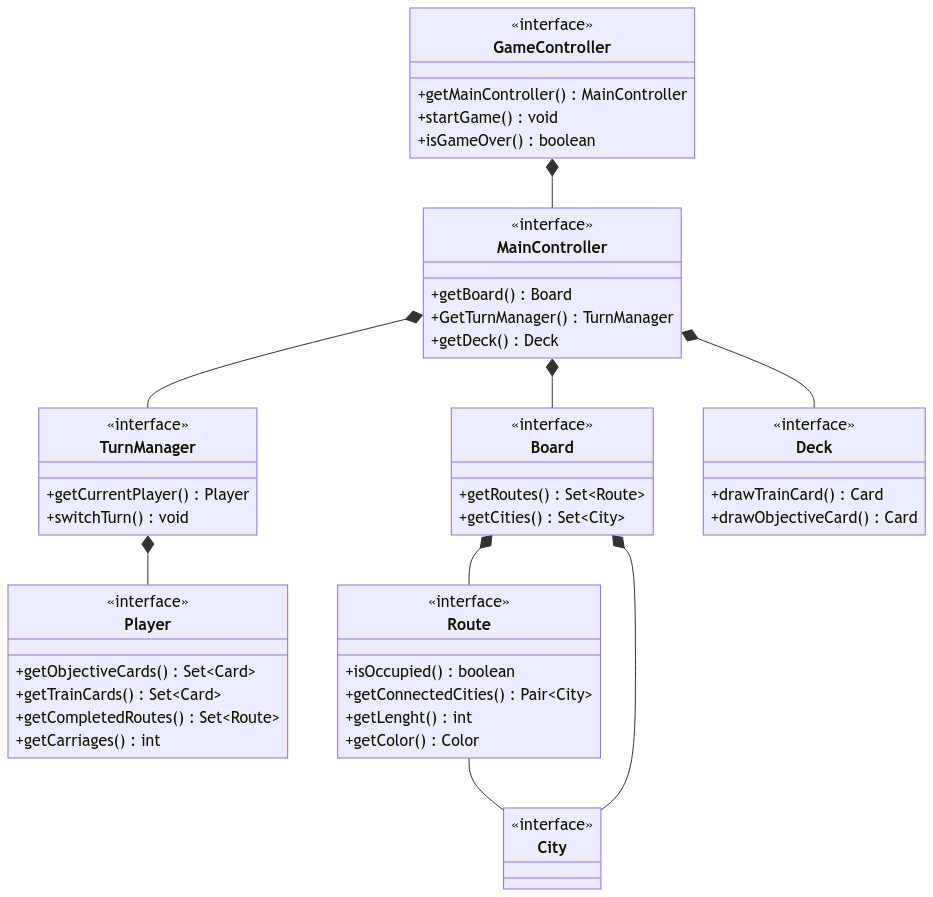
\includegraphics[scale=0.5]{UMLdomain.png}
\caption{Schema UML dell'analisi del problema, con rappresentate le entità principali ed i rapporti fra loro}
\label{img:analysisGraph}
\end{figure}

\chapter{Design}
\section{Architettura}
Per realizzare la nostra applicazione abbiamo voluto utilizzare un'architettura di tipo MVC. La parte di View è contenuta nel package \textit{it.unibo.view}. I giocatori possono interagire con il gioco pescando Carte, cambiando Turno e piazzando Treni tramite bottoni, forniti dalla libreria \textit{JavaFX}.  Tramite tali bottoni viene richiamato il Controller (package \textit{it.unibo.controller}), che gestisce la logica di gioco, ovvero gestione di Turni, Fase di gioco, lettura da file... Queste operazioni dipendono dalle classi del Model (package \textit{it.unibo.model}), che definisce "Route", "City", "Carriage", "Player" e altre classi. In questo modo possiamo cambiare l'implementazione delle Città, Carte o Rotaie senza dover apportare modifiche alla View o al Controller. Non ci sono dipendenze dirette tra View e Model, ciò renderebbe agile l'eventuale sostituzione di una delle due componenti.

\begin{figure}[H]
\centering{}
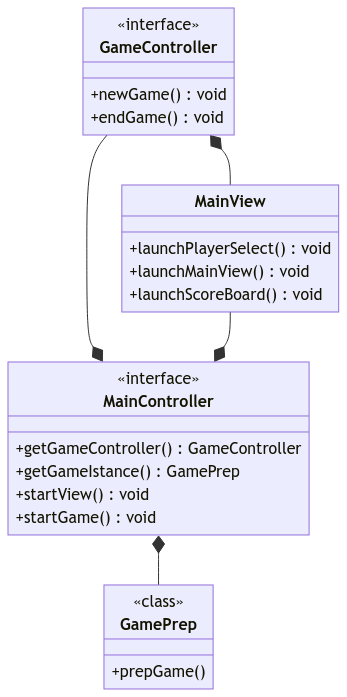
\includegraphics[scale=0.7]{UMLacrchitecture.png}
\caption{Schema UML dell'analisi del problema, con rappresentate le entità principali ed i rapporti fra loro}
\label{img:analysisGraph}
\end{figure}
\newpage


\section{Design dettagliato}
\subsection{Bergami Lorenzo}
\subsubsection{Lettura dati della mappa da file}
\begin{center}
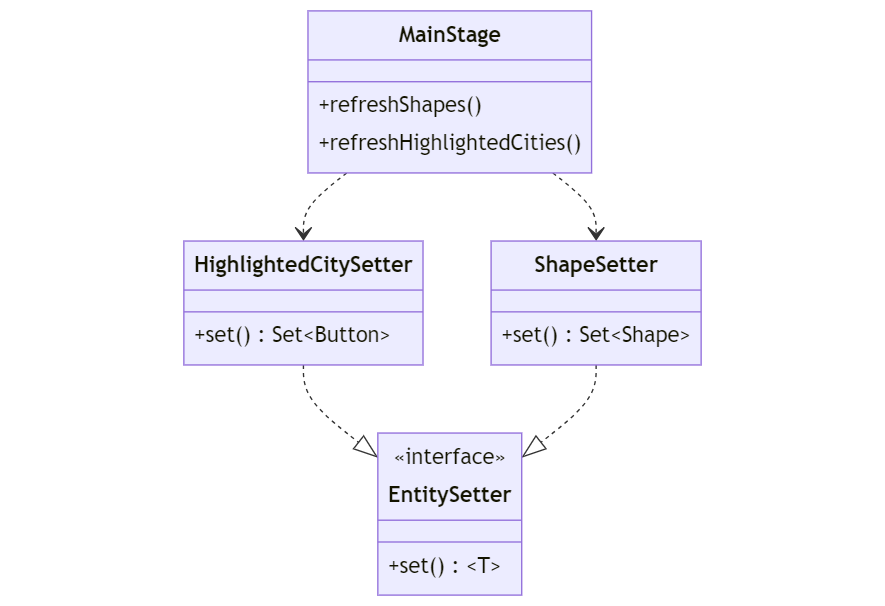
\includegraphics[scale=0.4]{mermaid-diagram-2024-02-22-222757.png}
\end{center}
\subsubsection{Problema}   Leggere dati relativi alle entità "City" e "Route" da file di configurazione

\subsubsection{Soluzione}  Linterfaccia ReaderController modella un lettore da file generico.
%
Tale interfaccia viene implementata da AbstractReaderController  (che definisce il costruttore), estesa poi da MapReaderController (lettura delle specifiche della mappa), RouteReaderController (lettura dati inerenti alle "Route") e CityReaderController (lettura dati inerenti alle "City"). 
%
Queste tre classi leggono ciascuna da un diverso file di configurazione in formato JSON tramite la libreria \textit{org.json.simple}, scelta siccome è molto semplice da utilizzare e consente di rappresentare facilmente strutture come liste di oggetti (nel nostro caso, "Route" o "City"). Questa scelta di design renderebbe molto facile l'aggiunta di altre mappe.
\newpage
%
\subsubsection{Generazione delle entità lette da file}

\begin{center}
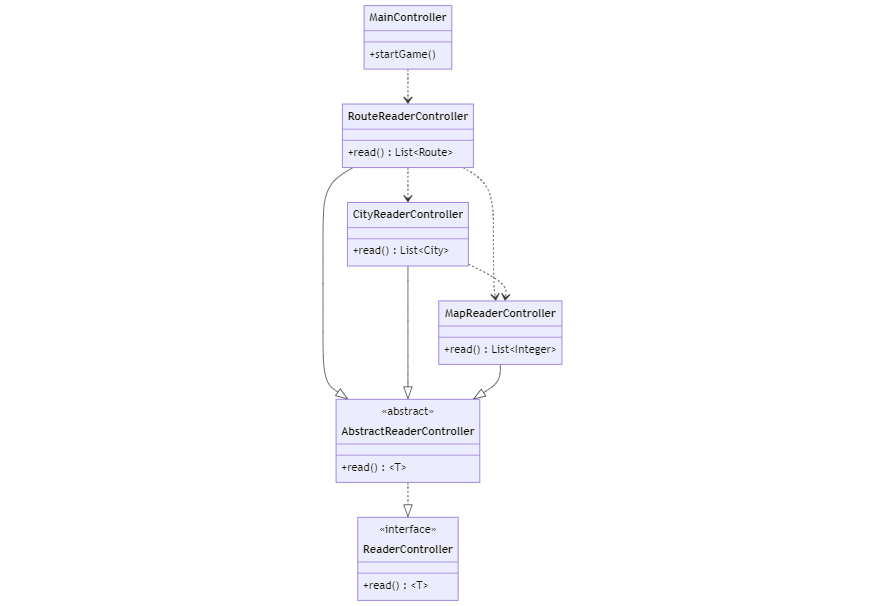
\includegraphics[scale=0.5]{mermaid-diagram-2024-02-22-222754.png}
\end{center}

\subsubsection{Problema}
Generare sulla mappa le entità lette da file

\subsubsection{Soluzione}
L'interfaccia EntitySetter modella un setter di entità generico. Viene implementata dalle classi HighlightedCitySetter e ShapeSetter. 
%
Si occupano rispettivamente di produrre bottoni per evidenziare le "City" che il giocatore corrente ha collegato riempiendo "Route", e di produrre i bottoni per selezionare le "Route" di tutta la mappa.
%
Queste classi sono necessarie per garantire una separazione netta tra View e Model, infatti invece di ricevere istanze di "City" o "Route" dal Controller ricevono nel primo caso una coppia di coordinate, mentre nel secondo istanze di "Region", una classe comune a tutto il progetto.

\subsubsection{Creazione dei file di configurazione}
\subsubsection{Problema}
Creare i file di configurazione dai quali leggere le specifiche della mappa e i dati relativi a "City" e "Route".
\subsubsection{Soluzione}
Ho creato 3 file in formato JSON, uno per la mappa, uno per "Route" e uno per "City". Ho scelto questo formato perchè consente di rappresentare e leggere facilmente strutture dati come liste di oggetti abritrari, esattamente ciò che ci serviva per descrivere l'insieme di "City" e "Route". Ho ricavato i dati dal file "EuropeMapLabeled.png".
\newpage
\subsection{Orazio Spina}
\subsubsection{Calcolo punteggi}
\begin{center}
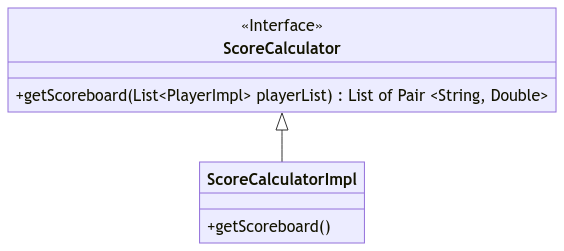
\includegraphics[scale=0.7]{scorecalculatorUML.png}
\end{center}

%
\subsubsection{Problema}
Calcolo dei punteggi finali della partita.

%
\subsubsection{Soluzione}
Si fa uso della classe ScoreCalculator per ottenere una lista di pair contenente la stringa con il nome del player e il relativo punteggio. Questi valori vengono ricevuti tramite una lista di giocatori che viene iterata per estrarne le informazioni.
\newpage
\subsubsection{Interfaccia Punteggi}
\begin{center}
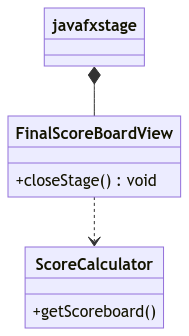
\includegraphics[scale=0.7]{interfacciapunteggiUML (1).png}
\end{center}

%
\subsubsection{Problema}
Mostrare nella view una schermata contenente la classifica finale con i relativi punteggi di ogni giocatore
%
\subsubsection{Soluzione}
Si fa uso di una classe che estende la classe Stage di JavaFX che si aggancia alla main application, contenente nel costruttore il codice necessario ad istanziare tutti gli elementi per creare una classifica.
\newpage
\subsubsection{Generazione casuale di obiettivi}
\begin{center}
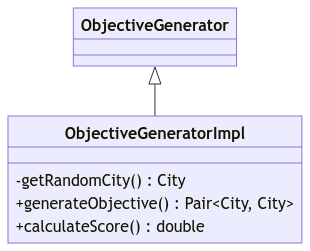
\includegraphics[scale=0.7]{objectivegeneratorUML (1).png}
\end{center}

%

\subsubsection{Problema}
Generare un obiettivo in maniera casuale, per obiettivo si intente una coppia di cittá presenti sulla mappa.
%
\subsubsection{Soluzione}
Si utilizza una classe ObjectiveGeneratorImpl che implementa la rispettiva interfaccia, il quale genera degli obiettivi casuali e calcola anche il loro valore in punteggio il quale é dato dal percorso piú corto per raggiungere la cittá di arrivo da quella di partenza, assicurandosi le due cittá non siano la stessa e che abbiano una distanza minima di tra di loro.
\newpage
\subsubsection{Scelta del numero di giocatori}
\begin{center}
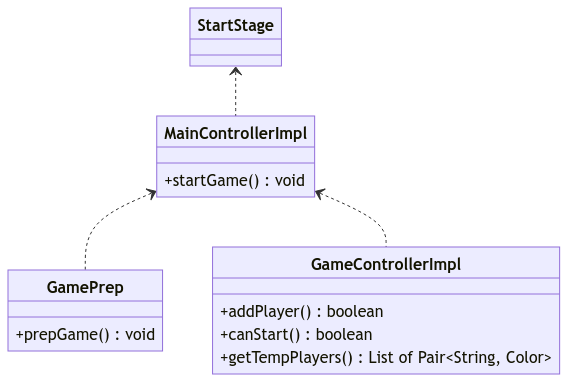
\includegraphics[scale=0.7]{numerodigiocatoriUML (1).png}
\end{center}

%
\subsubsection{Problema}
Dare la possibilitá di scegliere il numero di giocatori tra 2 e 6.
%
\subsubsection{Soluzione}
Si utilizza una classe StartStage che estende uno Stage della libreria JavaFX che all'interno ha un button che permette di aggiungere dei player dopo aver scelto nome (non é possibile inserire un nome vuoto o uguale ad uno giá presente) e colore (non é possibile avere due giocatori con lo stesso colore). Quando il numero di giocatori é sufficiente per iniziare la partita di attiverá un button che la fa iniziare. Ogni volta che si aggiunge un giocatore alla lista viene aggiunto ad una lista provvisoria al interno del game controller e viene chiesto se é possibile abilitare il pulsante di avvio partita. Una volta premuto il pulsante per avviare la partita viene invocato il MainCotrollerImpl che tramite la GamePrep genera un oggetto Player per ogni giocatore.
\newpage
\subsection{Massa Marco}
\subsubsection{Gestione dei turni e delle fasi di gioco}
\begin{center}
\includegraphics[scale=0.5]{PhaseManagerandTurnManagerUML.png}
\end{center}

%
\subsubsection{Problema}  
%
Gestire i turni dei giocatori e le fasi del turno di ogni giocatore.
%
\subsubsection{Soluzione} 
%
La classe TurnManager si occupa proprio di leggere la lista di giocatori, e da lì restituire all'occorrenza il giocatore corrente, la lista ordinata in base all'ordine del turno, e di cambiare turno, nella parte di controller la classe TurnController gestisce un turnmanager grazie al quale è quindi in grado di comunicare alla view e al resto dei controller le infomazioni relative alla gestione dei turni. Per quanto riguarda la gestione delle fasi di gioco la classe PhaseManager, tramite l'enumerazione delle tre fasi, si occupa di restituire l'attuale fase e di spostarsi alla successiva; anche per questa la classe PhaseController gestisce un phasemanager per comunicare le informazioni alla view. Entrambe vengono quindi gestite direttamente dentro alla classe MainController che ne trae le informazioni necessarie.
\newpage
\subsubsection{Pesca delle carte}
\begin{center}
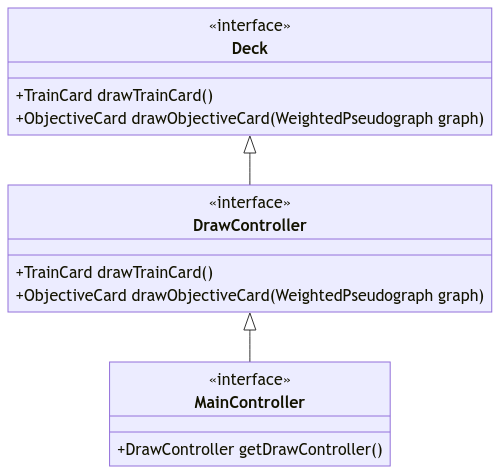
\includegraphics[scale=0.6]{drawControllerUML.png}
\end{center}
%
\subsubsection{Problema}  
Gestire la pesca delle carte.
%
\subsubsection{Soluzione} 
La classe Deck gestisce sia il mazzo delle carte Treno che il mazzo delle carte Obiettivo, mentre la classe DrawController passa le infomazioni dalla classe Deck al MainController.
\newpage
\subsubsection{Visualizzazione delle informazioni del giocatore corrente}
\begin{center}
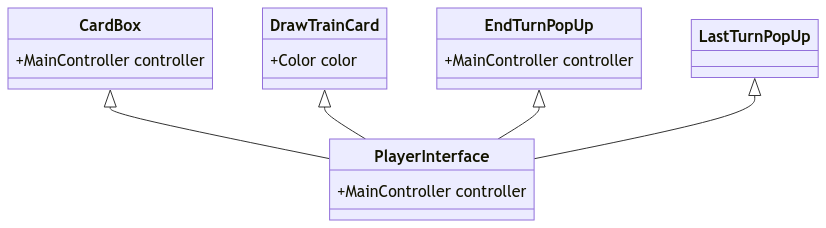
\includegraphics[scale=0.5]{viewUML.png}
\end{center}
%
\subsubsection{Problema}
%
Visualizzare le informazioni del giocatore e i pop-up relativi ai turni.
%
\subsubsection{Soluzione} 
%
La classe PlayerInterface gestisce tutte le informazioni relative al giocatore corrente, la classe CardBox ne gestisce la visualizzazione delle carte, mentre la classe DrawTrainCardPopUp mostra la carta Treno appena pescata, la classe EndTurnPopUp mostra il turno e il giocatore che deve giocare mentre la classe LastTurnPopUp informa il giocatore che sarà l'ultimo turno di gioco prima del calcolo dei punteggi.

\newpage
\subsection{Pietro Sbaraccani}
\subsubsection{Inserimento Carrozze e completamento delle tratte}
\begin{center}
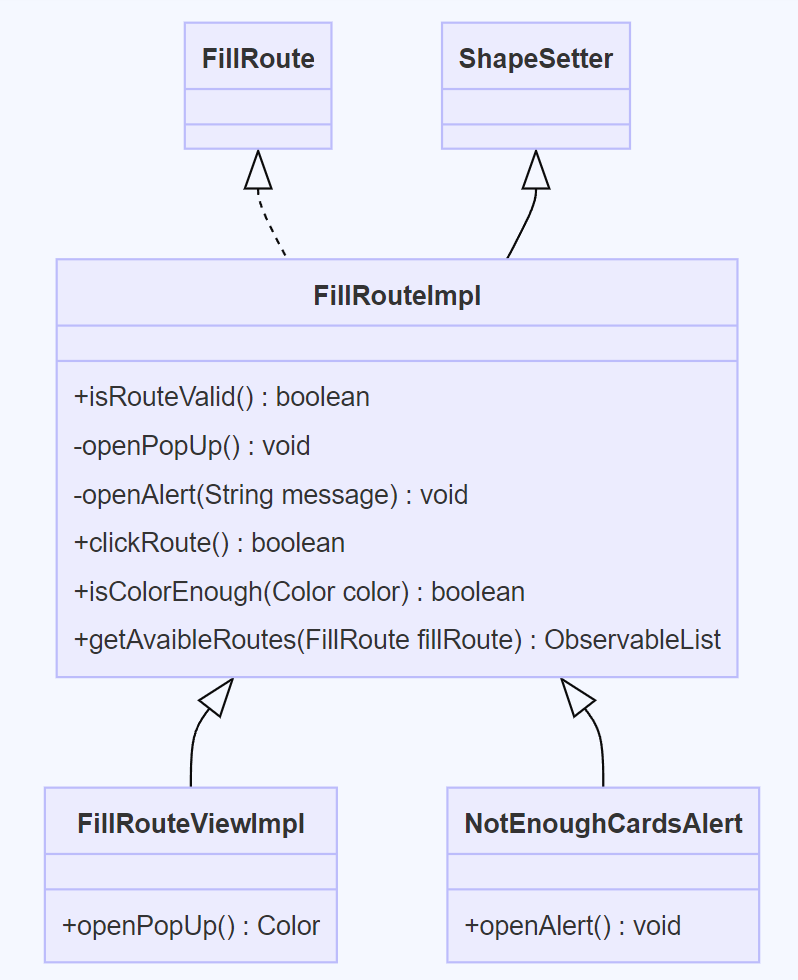
\includegraphics[scale=0.5]{fillroutecontrollerUML (1).png}
\end{center}
%
\subsubsection{Problema}
Calcolare le carrozze da rimuovere per riempire una Route
%
\subsubsection{Soluzione}
Si usa la classe FillRoute, quando una Shape viene clickata allora viene creata un'istanza di FillRouteImpl
e al costruttore viene passato il controller, il giocatore che ha clickato e la Regione che è stata clickata. Viene poi chiamata la funzione clickRoute() che distinguerà tutti i casi possibili ed eventualmente si occuperà di sottrarre i vagoni usati al giocatore che vuole riempire una Route.
%
\newpage
\subsubsection{Problema}
Il giocatore ha clickato una route di cui non può prendere il controllo
%
\subsubsection{Soluzione}
Se la route è già occupata o non si hanno abbastanza carrozze per riempirla, allora, viene chiamata una funzione openAlert() che si appoggierà alla classe NotEnoughCardsView per aprire una finestra di dialogo la quale comunicherà al giocatore che non è possibile riempire quella Route.
%
%
\newpage
\subsubsection{Problema}
Il giocatore ha clickato una route di cui può prendere il controllo immediatamente
%
\subsubsection{Soluzione}
Se la route ha un colore diverso dal grigio e il giocatore ha abbastanza carte Carrozza di quel colore oppure ha abbastanza carte Carroza di quel colore sommate ai jolly, la classe FillRouteImpl si occuperà di rimuovere le carte del giocatore (prima le colorate, poi eventualmente i jolly) e segnare come occupata la Route.
%
\newpage
%
\subsubsection{Problema}
Il giocatore ha clickato una route grigia
%
\subsubsection{Soluzione}
In questo caso bisogna fare scegliere all'utente il colore delle carrozze che si vogliono utilizzare, mi appoggierò per cui alla classe FillRouteViewImpl a cui nel costruttore passerò la lista di tutti i colori disponibili per il piazzamento delle tratta calcolati nella classe FillRouteImpl.
Si apre quindi una finestra di dialogo che permette al giocatore di scegliere quale colore vuole utilizzre, il controllo viene passato poi di nuovo a FillRouteImpl che si occuperà di rimuovere le carrozze scelte dall'utente e segnare come occupata quella Route.
Nel caso in cui non si abbiano abbastanza carrozze di nessun colore, allora come nel caso delle route colorate vivne aperta una finestra di dialogo che comunica l'impossibilità di prendere il controllo di quella Route.
%
\newpage

\chapter{Sviluppo}
\section{Testing automatizzato}

Abbiamo effettuato testing automatizzato tramite \textit{JUnit 5}. Sono state realizzate 5 classi:
\begin{itemize}
    \item TestGamePrep: verifica la corretta inizializzazione dei giocatori (nome, colore, numero di carrozze) e del grafo (numero di "City" e "Route").
    \item TestObjectiveGeneration: testa  se gli obiettivi generati sono diversi e se la distanza coperta tra gli estremi dell'obiettivi è maggiore della distanza minima.
    \item TestReaderController: controlla la corretta letture delle specifiche della mappa, delle entità "Città" e "Route", che rispettivamente dipende da MapReaderController, CityReaderController e RouteReaderController.
    \item TestScoreCalculator: verifica la corretta assegnazione dei punteggi al termine della partita.
    \item TestTurnAndPhase: controlla il corretto funzionamento della logica di "Turno", l'alternarsi dei giocatori e la logica di "Fase di Gioco" nel turno di uno stesso giocatore.
\end{itemize}

\section{Note di sviluppo}

\subsection{Orazio Spina}
\subsubsection{Utilizzo di Stream e lambda expressions}
Usato in vari casi, riporto un esempio: \url{https://github.com/TaricSpears/OOP23-tckt-to-rd/blob/master/src/main/java/it/unibo/model/scorecalculator/impl/ScoreCalculatorImpl.java}

\subsubsection{Utilizzo di wrapper in delle classi}
Usati in due casi. Ad esempio: \url{https://github.com/TaricSpears/OOP23-tckt-to-rd/blob/master/src/main/java/it/unibo/model/player/impl/PlayerImpl.java}

\subsubsection{Utilizzo della libreria JavaFX}
Un esempio é: \url{https://github.com/TaricSpears/OOP23-tckt-to-rd/blob/master/src/main/java/it/unibo/view/ObjectiveBox.java}

\subsubsection{Utilizzo della libreria JGraphT}
Usata in varie implementazioni, un esempio é la classe common \url{https://github.com/TaricSpears/OOP23-tckt-to-rd/blob/master/src/main/java/it/unibo/commons/GraphCopier.java}
\newpage
\subsection{Massa Marco}
\subsubsection{Utilizzo di librerie esterne di JavaFX}
Utilizzo di diverse librerie di JavaFX per migliorare la view del gioco, come aggiungere le immagini di sfondo, o la visualizzazione della carta pescata. Di seguito alcuni esempi:

\begin{itemize}
    \item Permalink: \url{https://github.com/TaricSpears/OOP23-tckt-to-rd/blob/master/src/main/java/it/unibo/view/DrawTrainCardPopUp.java#L50-L53}
    \item Permalink: \url{https://github.com/TaricSpears/OOP23-tckt-to-rd/blob/master/src/main/java/it/unibo/view/EndTurnPopUp.java#L34-L36}
    \item Permalink: \url{https://github.com/TaricSpears/OOP23-tckt-to-rd/blob/master/src/main/java/it/unibo/view/LastTurnPopUp.java#L16}
\end{itemize}
\newpage
\subsection{Bergami Lorenzo}
\subsubsection{Utilizzo di JavaFX}
Utilizzo di JavaFX per rappresentare "Route" e "City" sulla mappa di gioco:
\begin{itemize}
    \item Permalink: \url{https://github.com/TaricSpears/OOP23-tckt-to-rd/blob/master/src/main/java/it/unibo/view/entitysetter/impl/HighlightedCitySetter.java}
    \item Permalink: \url{https://github.com/TaricSpears/OOP23-tckt-to-rd/blob/master/src/main/java/it/unibo/view/entitysetter/impl/ShapeSetter.java}
\end{itemize}
\subsubsection{Utilizzo di \textit{org.json.simple}}
Utilizzo della libreria esterna per leggere facilmente i file JSON di configurazione. L'ho scoperta dopo aver consultato il progetto "RisikOOP 2022". Un esempio:
\begin{itemize}
    \item Permalink: \url{https://github.com/TaricSpears/OOP23-tckt-to-rd/blob/master/src/main/java/it/unibo/controller/readercontroller/impl/RouteReaderController.java}
\end{itemize}
\subsubsection{Utilizzo di Optional}
\begin{itemize}
    \item Permalink: \url{https://github.com/TaricSpears/OOP23-tckt-to-rd/blob/master/src/main/java/it/unibo/commons/Region.java#L93-L98}
\end{itemize}
\subsubsection{Utilizzo di Record}
\begin{itemize}
    \item Permalink: \url{https://github.com/TaricSpears/OOP23-tckt-to-rd/blob/master/src/main/java/it/unibo/model/carriage/impl/Carriage.java}
\end{itemize}
\subsubsection{Utilizzo di Generici}
Utilizzo di generici per implementare una stessa interfaccia in classi che restituiscono oggetti diversi. Un esempio:
\begin{itemize}
    \item Permalink: \url{https://github.com/TaricSpears/OOP23-tckt-to-rd/blob/master/src/main/java/it/unibo/view/entitysetter/api/EntitySetter.java}
\end{itemize}
\newpage
\subsection{Sbaraccani Pietro}
\subsubsection{Utilizzo di JavaFX}
Utilizzo esteso di JavaFX,per esempio l'uso della ObservableList
\begin{itemize}
    \item Permalink: \url{https://github.com/TaricSpears/OOP23-tckt-to-rd/blob/master/src/main/java/it/unibo/controller/fillroutecontroller/impl/FillRouteImpl.java}
    \item Permalink: \url{https://github.com/TaricSpears/OOP23-tckt-to-rd/blob/master/src/main/java/it/unibo/view/fillroute/FillRouteViewImpl.java}
\end{itemize}
\section{Sviluppo comune}
Abbiamo iniziato lo sviluppato impostando assieme il Model dell'applicazione, principalmente le classi "Route", "City", "GamePrep" e "Player". 
\newpage
\chapter{Commenti finali}
\section{Autovalutazione e lavori futuri}
\subsection{Orazio Spina}
Il mio ruolo all'interno del gruppo era quello della generazione delle varie istanze dei player, il calcolo dei loro punteggi a fine gioco e la gestione del controllo delle interazioni tra i vari elementi del software. Ritengo di aver svolto un ruolo abbastanza importante per quanto riguarda la progettazione dell'architettura generale, verso la fine del progetto tutta via ci sono stati alcuni aspetti che hanno causato dei problemi. Tuttavia penso di aver svolto un buon lavoro. Tra i punti di forza inserirei quello di esser stato abbastanza abile nel risolvere i vari problemi che si sono presentati durante la realizzazione del progetto. Come punti di debolezza inserirei il fatto di aver sottostimato il carico di lavoro e la poca esperienza di lavoro in programmazione di gruppo. Le principali difficoltá riscontrate durante il progetto sono:
\begin{itemize}
 \item Utilizzo di JavaFX: una libreria mai usata e non vista a lezione. Sopratutto agli inizi non é stato facile capire quale componente fosse piú adatto alle mie necessitá e capire come posizionare gli elementi nello spazio.
 \item Utilizzo di Git: apparte l'utilizzo per le esercitazioni di laboratorio non lo avevo mai usato, ho trovato difficoltá nel suo utilizzo in maniera efficente.
 \item Organizzazione del progetto: organizzare le fasi iniziali del progetto, come l'analisi del dominio e modellare come le varie entitá dovevano interagire tra di loro.
\end{itemize}
\subsection{Massa Marco}
Sono soddisfatto del lavoro svolto insieme agli altri membri del gruppo, grazie a questo tipo di progetto ho potuto capire quanto è importante il lavoro di squadra al fine di raggiungere lo stesso obiettivo finale. Il lavoro di gruppo è stato senza dubbio facilitato dallo strumento Github, che grazie alla sua efficienza ha velocizzato lo sviluppo dele parti comuni. La difficoltà più grande che ho avuto è capire il funzionamento di Javafx, che prima non conoscevo. Infine, desidero sottolineare l'importanza della comunicazione e della collaborazione all'interno del gruppo. La capacità di ascolto attivo e di scambio di idee ha giocato un ruolo fondamentale nel superare le sfide.
\subsection{Sbaraccani Pietro}
Mi sono occupato dell'interazione tra Giocatore e Mappa per il piazzamento di Carrozze su Route.
Il mio punto di forza è stata la conoscenza del gioco, che mi ha aiutato nella fase iniziale; spero di essere stato d'aiuto al gruppo a visualizzare con chiarezza il dominio dell'applicazione.\\
Ho trovato difficoltà invece a rispettare le dipendenze tra Model, View e Controller.
Questo progetto mi ha dato l'occasione di imparare a utilizzare GitHub e JavaFX, in più ho sviluppato una conoscenza più profonda dell'architettura MVC.\\
Avrei preferito svolgere il progetto con più calma, in modo da ponderare meglio le scelte implementative; ciononostante sono soddisfatto sia del lavoro che ho svolto singolarmente sia del lavoro che abbiamo svolto come gruppo.
\subsection{Bergami Lorenzo}
Il mio ruolo è stato la creazione dei file di configurazione, la conseguente lettura e la generazione delle entità di gioco da mostrare a video.
Le sfide principali sono dipese dalla vastità del lavoro: non mi ero mai dedicato a progetti veri e propri, dunque l'inizio è stato abbastanza disorientante; grazie al gruppo sono riuscito a inquadrare il mio compito e penso di averlo raggiunto con successo. Come punto di debolezza direi che non sono riuscito ad avere fin dall'inizio una buona visione d'insieme, che avrebbe portato forse a scelte di desing più eleganti.
 Sono soddisfatto del mio operato, anche perchè ho imparato a usare GitHub nel contesto di un gruppo e ho usato librerie come \textit{JavaFX} e \textit{org.json.simple} che prima del progetto non conoscevo.
\newpage

\appendix
\chapter{Guida utente}

All'avvio dell'applicazione viene mostrata una schermata di player selection, in cui si può aggiungere fino a 6 giocatori necessariamente distinti per nome e colore. Fatto ciò si può iniziare la partita.
A partita iniziata la mappa è riempita di rotaie inutilizzate. Il giocatore deve seguire le indicazioni testuali mostrate in alto a destra:
\begin{itemize}
    \item Pesca: premere i bottoni "Draw"
    \item Numero carrozze: ogni giocatore inizia la partita con 45 Carrozze, dunque può riempire 45 "unità" delle rotaie. Il numero di Carrozze rimaste è mostrato sopra il bottone "Reveal Objectives".
    \item Numero carte in Mano: il numero sottostante l'immagine di una carta indica il numero di carte di quel colore: per esempio, con 2 carte Rosse si può occupare una tratta rossa lunga due unità.
    \item Piazzare treni: clickare sulla mappa la rotaia che si vuole occupare (si accenderanno le città collegate dalla tratta e la tratta sarà evidenziata del colore del giocatore). L'operazione va a buon fine se la fase di gioco è corretta, se il giocatore ha sufficienti Carte Treno adatte alla tratta e se ha sufficienti Carrozze.
    \item Mostrare obiettivi: siccome gli obiettivi sono intesi come visibili solo dal giocatore corrente, premere il bottone "Reveal Objectives".
    \item Passare il turno: clickare bottone "End Turn".
    \item Consultare Regole: premere bottone "Rules".
\end{itemize}
Quando almeno un giocatore ha meno di 3 Carrozze, la partita termina. A questo punto viene mostrata la classifica. Si può iniziare una nuova partita oppure chiudere l'applicazione.

\end{document}
